\documentclass[12pt]{article}
\usepackage[utf8]{inputenc}
\usepackage[T5]{fontenc} % For Vietnamese characters
\usepackage{lmodern} % Modern font
\usepackage{amsmath}
\usepackage{graphicx}
\usepackage[colorlinks=false, hidelinks]{hyperref}
\usepackage{float} % For [H] placement of figures
\usepackage{longtable} % For tables that span multiple pages
\usepackage{booktabs} % For professional-looking tables
\usepackage{multirow} % For multirow cells in tables
\usepackage{geometry} % For page margins
\geometry{a4paper, left=2.5cm, right=2.5cm, top=2.5cm, bottom=2.5cm}



\begin{document}



\begin{titlepage}
    \centering % Center all content on the title page

    % Top section: Institute, Faculty, Department
    % Using Huge and Large for prominence, and \\ for line breaks, \[...] for vertical spacing
    {\large\bfseries POSTS AND TELECOMMUNICATIONS\\[0.2cm] INSTITUTE OF TECHNOLOGY} \\[0.5cm] 
    {\large\bfseries FACULTY OF INFORMATION TECHNOLOGY I} \\[0.5cm] % Reduced from \Large to \large, increased spacing to 0.7cm
    {\normalsize\bfseries DEPARTMENT OF PYTHON PROGRAMMING} \\[2cm] % Reduced from \large to \normalsize, original spacing (2cm) is kept as it's a larger break

    % Main Report Title
    
    % Using Huge and bfseries for main report title

    % Logo section
    \begin{center}
    % Adjust width if needed, make sure the image path is correct relative to your .tex file
    
\includegraphics[width=5cm]{Screenshots/image1 .png} % Path to your PTIT logo image
    \end{center}
    \vspace{0.5cm} % Vertical space after logo
    {\Huge\bfseries ASSIGNMENT 2} \\[2.5cm]
    

    % Instructor and Student Information - styled to match flushleft of snippet 2, but keeping tabular for alignment
    \begin{flushleft} % Align this block to the left
    \large % Set font size to large for this block
    \begin{tabular}{ll} % Using a two-column tabular for clean alignment of labels and values
    \textbf{Lecturers of the Department} & : KIM NGOC BACH \\
    \textbf{Class} & : D23CQCE04 - B \\
    \textbf{Full name} & : TRAN TRUNG HIEU - B23DCCN312 \\ % Keep \textbf{Full name} as requested
    & : NGUYEN HUU NIEM - B23DCCE076 \\ % Aligned under the previous Full name
    \end{tabular}
    \end{flushleft}
    \vspace{1cm} % Space after info block

    \vfill % Fill remaining vertical space to push date to bottom

    % Bottom section: City and Year
    {\large Ha Noi – 2025} % Set font size to large for date/city

\end{titlepage}

\pagestyle{plain} % Reset page style for main content

\newpage
\section*{PREFACE}
In today's digital age, computer vision has become an important field, contributing to the development of many practical applications from medicine, manufacturing to self-driving cars and security. At the heart of computer vision is the ability for computers to "understand" and interpret information from digital images or videos. One of the most basic and fundamental problems in this field is image classification. Image classification requires computers to assign a specific label or category to an input image, simulating human recognition capabilities.
\\
\\
With the explosion of Deep Learning, especially the emergence and development of Convolutional Neural Networks (CNNs), the performance of image classification systems has been raised to a new level, far surpassing traditional methods. To understand and compare the effectiveness of neural network architectures, this exercise focuses on implementing and evaluating two main types of models: Multi-Layer Perceptron (MLP) and Convolutional Neural Networks (CNN), on the CIFAR-10 benchmark dataset.
\\
\\
This paper details the data preparation process, architecture design and implementation of MLP and CNN, training and testing process, and analysis and comparison of the results. Through this, the paper aims to clarify the performance differences and outstanding advantages of CNN compared to MLP in image classification. The entire implementation process is based on the PyTorch library, a powerful and flexible tool in deep learning research and development.
\\
\\
We hope that this report will provide a comprehensive and in-depth look at the application of MLPs and CNNs in image classification, while also affirming the importance of choosing the right model architecture given the nature of the data and the problem.
\\
\\
Best regards!


\newpage
\tableofcontents

\newpage
\section{INTRODUCTION}
\subsection{Overview of the image classification problem}
Image classification is one of the most fundamental and important tasks in the field of computer vision. The main goal of image classification is to assign a specific label to an image based on its content. This process typically involves extracting features from the image and using machine learning or deep learning algorithms to learn patterns related to each object class. Image classification applications are diverse and have a significant impact on many industries, including:
\begin{itemize}
    \item Object recognition: Used in self-driving cars to detect pedestrians, traffic, and road signs.
    \item Medical image analysis: Supports disease diagnosis from X-ray and MRI images.
    \item Image search: Finds similar images based on content.
    \item Quality control: In production to detect product defects.
\end{itemize}
The development of Deep Learning, especially Convolutional Neural Networks (CNNs), has made significant breakthroughs in the performance of image classification systems.

\subsection{Introduction to CIFAR-10 dataset}
This exercise uses the CIFAR-10 dataset, a popular and widely used dataset in research and development of computer vision algorithms. CIFAR-10 has the following salient features:
\begin{itemize}
    \item Size: Includes 60,000 color images (RGB) with a compact size of 32x32 pixels.
    \item Classify: Divided into 10 different object classes, each with 6,000 images.
    \item Classes: The 10 classes include: 'plane', 'car', 'bird', 'cat', 'deer', 'dog', 'frog', 'horse', 'ship', and 'truck'.
    \item Split episode: The dataset is pre-split into 50,000 training images and 10,000 test images.
\end{itemize}

\subsection{Objectives and scope of the report}
The main objective of this paper is to perform image classification task on CIFAR-10 dataset by building, training and evaluating two types of neural network architectures:
\begin{itemize}
    \item Multilayer Feedforward Neural Network (MLP): A basic network with 3 hidden layers.
    \item Convolutional Neural Network (CNN): An image-specific network with 3 convolutional layers.
\end{itemize}
The scope of the report will include steps from data preparation, model architecture design, training process, testing and performance evaluation of each model. Finally, we will conduct a detailed comparison and discussion of the results achieved between MLP and CNN to clarify the advantages and disadvantages of each architecture in this problem.

\subsection{Tools and libraries used}
The entire implementation and analysis process is done in Python programming language. The main libraries used include:
\begin{itemize}
    \item PyTorch: The main framework for building and training neural network models.
    \item torchvision: PyTorch's data and computer vision model support library, used to load the CIFAR-10 dataset and apply image transformations.
    \item torch.nn: The module contains the classes for building neural networks.
    \item torch.optim: Module containing optimizer algorithms.
    \item matplotlib.pyplot: To draw graphs (learning curves).
    \item numpy: Support array calculations.
    \item sklearn.metrics: To calculate and display confusion matrix and classification report.
    \item seaborn: To visualize the confusion matrix more beautifully.
\end{itemize}

\section{DATA PREPARATION}
Data preparation and preprocessing is a crucial step to ensure effective model learning, enhance generalization ability, and minimize training issues.

\subsection{Load and transform data}
The CIFAR-10 dataset is downloaded and the necessary transformations are applied to both the training and testing/validation sets.

\subsubsection{Data Augmentation}
To improve the generalizability of the model and reduce overfitting, Data Augmentation techniques are applied to the training set. These transformations help the model get used to many variations of the same object:
\begin{itemize}
    \item \texttt{transforms.RandomCrop(32, padding=1)}: Randomly crops a 32x32 pixel portion of the image after adding 1 pixel of padding around the image. This helps the model not to be too dependent on the exact location of the object in the image and get used to different parts of the object.
    \item \texttt{transforms.RandomHorizontalFlip()}: Randomly flips the image horizontally. This is a simple but effective transformation that helps the model learn that the object can appear in any horizontal direction.
    \item \texttt{transforms.ToTensor()}: Converts an image from a PIL Image or NumPy array format to a PyTorch Tensor. Tensor is the data format that PyTorch uses to perform calculations on the GPU or CPU.
    \item \texttt{transforms.Normalize((0.5, 0.5, 0.5), (0.5, 0.5, 0.5))}: Normalizes the pixel values of each color channel (RGB) to the range [-1, 1]. This normalization helps the input values of the network have the same scale, thereby speeding up the convergence of the training process and improving the performance of the model.
\end{itemize}

\subsubsection{Data transformation for testing/validation set}
For the test and validation sets, the goal is to accurately evaluate the real-world performance of the model on unseen data. Therefore, we only apply the necessary transformations to format and normalize the data, without using data augmentation techniques:
\begin{itemize}
    \item \texttt{transforms.ToTensor()}: Converts an image to a PyTorch Tensor.
    \item \texttt{transforms.Normalize((0.5, 0.5, 0.5), (0.5, 0.5, 0.5))}: Normalizes pixel values to the range [-1, 1].
\end{itemize}

\subsection{Data set division}
The downloaded CIFAR-10 dataset has been divided into 50,000 training images and 10,000 testing images. To ensure that the model validation process is objective and not influenced by the training data, we further divide the original training set into a training set and a validation set:
\begin{itemize}
    \item Training set: Downloaded and applied \texttt{transform\_train}.
    \item Test set: Downloaded and applied \texttt{transform\_test}.
    \item Validation split: 10\% of the data from the \texttt{trainset} is used as the validation set (\texttt{val\_dataset}), and the remaining 90\% is the actual training set (\texttt{train\_dataset}).
    \item Training set size: 45,000 images.
    \item Audit set size: 5,000 images.
    \item Test set size: 10,000 images.
\end{itemize}

\subsection{DataLoader Configuration}
To manage and load data in batches during training and testing, we use PyTorch's DataLoader:
\begin{itemize}
    \item Batch Size: \texttt{batch\_size} is set to 128. Batch size affects training speed (larger batches are usually faster) and gradient stability (smaller batches usually have noisier gradients).
    \item Data Shuffle: \texttt{shuffle=True} is set to the \texttt{trainloader} to ensure each epoch of data is randomly shuffled, which helps the model not learn the order of the data and improves generalization ability.
    \item Multithreading: \texttt{num\_workers=2} is used to load data in parallel, which helps speed up data loading and avoids CPU/GPU waiting due to slow data loading.
    \item \texttt{trainloader}: DataLoader for the training set.
    \item \texttt{valloader}: DataLoader for the validation set.
    \item \texttt{testloader}: DataLoader for the test set.
\end{itemize}

\subsection{Object classes in CIFAR-10}
CIFAR-10 consists of 10 different object classes. Knowing these classes helps us better understand the problem and analyze the results later, especially in the confusion matrix. These classes are defined as a tuple in the source code: \\
\textbf{Classes} = ('plane', 'car', 'bird', 'cat', 'deer', 'dog', 'frog', 'horse', 'ship', 'truck')

\section{MODEL ARCHITECTURE}
In this section, we will detail the architecture of the two neural network models built: MLP and CNN. Both models are implemented using PyTorch.

\subsection{Multi-Layer Perceptron (MLP)}
\subsubsection{Overview of MLP}
MLP, also known as feedforward neural network, is one of the most basic neural network architectures. MLP consists of an input layer, one or more hidden layers, and an output layer. The neurons between the layers are fully connected, and information flows only in one direction from the input layer to the output layer. MLP is suitable for problems where the input data can be represented as a flat vector. However, when processing images, MLP is often not as effective as CNN because it does not take advantage of the spatial structure of pixels.

\subsubsection{MLP architecture design}
The MLP model is designed to process CIFAR-10 images. The input is a 32x32 pixel (3 channel) color image, which will be flattened into a 1D vector.
\begin{itemize}
    \item \textbf{Flatten class (\texttt{nn.Flatten()}):} The first layer in the model is responsible for converting the input tensor from (batch\_size, channels, height, width) to (batch\_size, channels * height * width). For the CIFAR-10 image, the input size will be $3 \times 32 \times 32 = 3072$ features.
    \item \textbf{Fully Connected (FC) or Linear (\texttt{nn.Linear}) classes:} The model uses 3 FC layers:
    \begin{itemize}
        \item \texttt{self.fc1 = nn.Linear(3 * 32 * 32, 512)}: The first hidden layer, receives 3072 features from the Flatten layer and transforms them into 512 features.
        \item \texttt{self.fc2 = nn.Linear(512, 256)}: Second hidden layer, takes 512 features from the previous layer and transforms them into 256 features.
        \item \texttt{self.fc3 = nn.Linear(256, num\_classes)}: Output layer, takes 256 features and produces \texttt{num\_classes} (10) outputs, corresponding to the scores (logits) for each class.
    \end{itemize}
    \item \textbf{ReLU activation function (\texttt{nn.ReLU()}):} Applied after the \texttt{fc1} and \texttt{fc2} layers. The ReLU (Rectified Linear Unit) function introduces nonlinearity into the model, helping the network learn more complex relationships in the data. Without the nonlinear function, MLPs can only learn linear relationships.
    \item \textbf{Dropout (\texttt{nn.Dropout(p=0.3)}):} Two Dropout layers are added after each ReLU activation function (\texttt{self.relu1} and \texttt{self.relu2}). Dropout is an effective regularization technique to combat overfitting. During training, a random percentage (p=0.3, or 30\%) of neurons are “disconnected” (temporarily not involved in the computation) in each data pass. This forces the network to learn more robust representations that are less dependent on any particular neuron.
\end{itemize}

\subsubsection{Forward Pass Function of MLP}
The forward function defines the flow of data through the network, from input to output:
\begin{figure}[H]
    \centering
    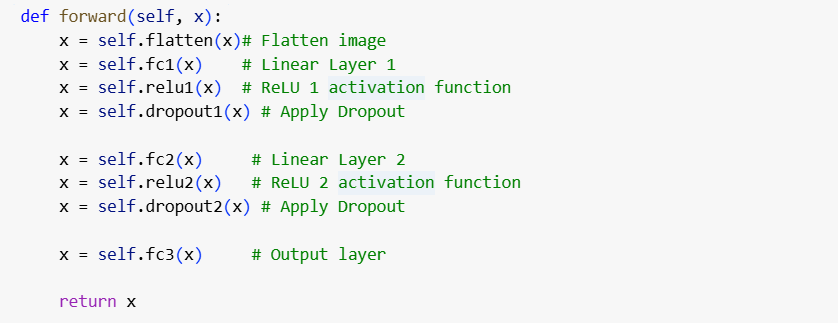
\includegraphics[width=0.8\textwidth]{Screenshots/Ảnh chụp màn hình 2025-05-23 221832.png} % Replace with your image path
    \caption{MLP Forward Pass Function}
    \label{fig:mlp_forward_pass}
\end{figure}

\subsection{Convolutional Neural Network (CNN)}
\subsubsection{Overview of CNN}
CNNs are a type of neural network that is particularly effective at processing grid-structured data such as images. Unlike MLPs, CNNs take advantage of the spatial structure of images through convolutional layers. These layers are capable of automatically learning filters to extract important features from the data, from low-level features (edges, corners) to high-level features (parts of objects).

\subsubsection{CNN architecture design}
The CNN model is designed with 3 consecutive convolutional blocks, followed by a Fully Connected layer.
\begin{itemize}
    \item \textbf{Convolutional and Pooling layers (\texttt{self.conv\_layers}):}
    \begin{itemize}
        \item \textbf{Convolution block 1:}
        \begin{itemize}
            \item \texttt{nn.Conv2d(3, 32, kernel\_size=3, padding=1)}: Receive RGB image (3 channels), apply 32 3x3 filters. \texttt{padding=1} helps keep the spatial size after convolution. Output: 32 channels, spatial size 32x32.
            \item \texttt{nn.ReLU()}: Nonlinear activation function.
            \item \texttt{nn.MaxPool2d(kernel\_size=2, stride=2)}: Perform Max Pooling with a 2x2 window and stride 2, reducing the spatial size by half. Output: 32 channels, 16x16.
        \end{itemize}
        \item \textbf{Convolution block 2:}
        \begin{itemize}
            \item \texttt{nn.Conv2d(32, 64, kernel\_size=3, padding=1)}: Receive 32 channels from previous layer, apply 64 3x3 filters. Output: 64 channels, 16x16.
            \item \texttt{nn.ReLU()}: Nonlinear activation function.
            \item \texttt{nn.MaxPool2d(kernel\_size=2, stride=2)}: Reduce the space size. Output: 64 channels, 8x8.
        \end{itemize}
        \item \textbf{Convolution block 3:}
        \begin{itemize}
            \item \texttt{nn.Conv2d(64, 128, kernel\_size=3, padding=1)}: Receive 64 channels from previous layer, apply 128 3x3 filters. Output: 128 channels, 8x8.
            \item \texttt{nn.ReLU()}: Nonlinear activation function.
            \item \texttt{nn.MaxPool2d(kernel\_size=2, stride=2)}: Reduce the final space size. Output: 128 channels, 4x4.
        \end{itemize}
    \end{itemize}
    \item \textbf{Calculate the input size for the FC layer:} After 3 layers of Max Pooling, the spatial size of the image has been reduced from 32x32 to 4x4. So the input size for the final Fully Connected layer will be $128 \times 4 \times 4 = 2048$ features. \texttt{self.fc\_input\_dim = 128 * 4 * 4}.
    \item \textbf{Dropout (\texttt{self.dropout\_fc = nn.Dropout(p=0.3)}):} A Dropout layer with a scale of 0.3 is added before the final Fully Connected layer. This helps prevent overfitting by randomly ignoring some of the features learned from the convolutional layers, forcing the model to rely on many different features to make predictions.
    \item \textbf{Final Fully Connected (FC) class (\texttt{self.fc}):}
    \begin{itemize}
        \item \texttt{self.fc = nn.Linear(self.fc\_input\_dim, num\_classes)}: This layer takes a flattened vector (2048 features) and produces 10 outputs (logits), corresponding to the 10 object classes of CIFAR-10.
    \end{itemize}
\end{itemize}

\subsubsection{Forward Pass Function of CNN}
The forward function defines the data flow through the CNN network:
\begin{figure}[H]
    \centering
    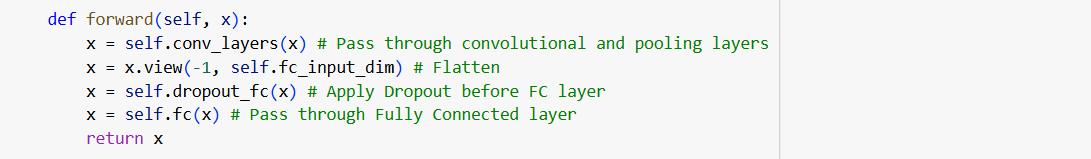
\includegraphics[width=0.8\textwidth]{Screenshots/Ảnh chụp màn hình 2025-05-23 222100.png} % Replace with your image path
    \caption{CNN Forward Pass Function}
    \label{fig:cnn_forward_pass}
\end{figure}

\section{TRAINING AND TESTING PROCESS}
To ensure fairness and objectivity in evaluating the performance of the two models, the training and testing processes are set up according to a common configuration and use pre-defined functions.

\subsection{General configuration for training}
\begin{itemize}
    \item \textbf{Device:} The model is trained on GPU (cuda) if available to speed up the computation, otherwise it automatically switches to CPU. During code execution, the device used is cuda.
    \item \textbf{Number of Epochs (\texttt{num\_epochs}):} Both models will be trained for 20 epochs. This number of epochs is an important hyperparameter that affects the training time and convergence ability of the model.
    \item \textbf{Learning rate (\texttt{learning\_rate}):} The learning rate is set to 0.001. This is a common value that controls how quickly the model updates its weights during optimization.
    \item \textbf{Loss function (Criterion):} \texttt{nn.CrossEntropyLoss()} is used as the loss function. This is the standard choice for multiclass classification problems in PyTorch, combining the softmax function and negative log-likelihood loss.
    \item \textbf{Optimizer:} \texttt{optim.Adam()} is used to update the model weights. Adam is a popular adaptive optimization algorithm that typically provides good performance and converges quickly.
\end{itemize}

\subsection{Training function (\texttt{train\_model})}
The \texttt{train\_model} function is designed to manage the entire process of training and validating a model over epochs:
\begin{itemize}
    \item \textbf{Transfer model to device:} \texttt{model.to(device)} ensures that the model and data are processed on the same device (GPU or CPU).
    \item \textbf{Historical Archives:} The lists \texttt{train\_losses}, \texttt{val\_losses}, \texttt{train\_accuracies}, and \texttt{val\_accuracies} are initialized to record the loss and accuracy of both the training and validation sets over each epoch. This is necessary to plot the learning curve.
    \item \textbf{Epoch Loop:}
    \begin{itemize}
        \item \textbf{Training mode:} \texttt{model.train()} is called at the beginning of each epoch to put the model into training mode. In this mode, the Dropout layers will run and the model parameters will be updated.
        \item \textbf{Batch Training:} For each batch of data from \texttt{train\_loader}:
        \begin{itemize}
            \item Data (\texttt{images}, \texttt{labels}) are transferred to the device.
            \item Perform a straight pass (\texttt{model(images)}) to get the model output.
            \item Loss calculation (\texttt{criterion(outputs, labels)}).
            \item Delete the old gradient (\texttt{optimizer.zero\_grad()}).
            \item Backpropagate (\texttt{loss.backward()}) to calculate the gradient.
            \item Update weights (\texttt{optimizer.step()}).
            \item Calculate the running loss and training set accuracy for the current epoch.
        \end{itemize}
        \item \textbf{Evaluation mode:} \texttt{model.eval()} is called to switch the model to evaluation mode. In this mode, Dropout layers will be disabled and parameters will not be updated.
        \item \textbf{Rating on the review set:} For each batch of data from \texttt{val\_loader}, and use \texttt{with torch.no\_grad():} to not calculate the gradient:
        \begin{itemize}
            \item Data is transferred to the device.
            \item Perform straight transmission.
            \item Compute loss and precision for the validation set of the current epoch.
        \end{itemize}
        \item \textbf{Print Epoch results:} Print out the loss and accuracy on both the training and validation sets of the current epoch to track progress.
    \end{itemize}
    \item \textbf{Complete training:} After all epochs are completed, the message "Training complete." is printed.
    \item The function returns the collected loss and accuracy lists.
\end{itemize}

\subsection{Test function (\texttt{test\_model})}
The \texttt{test\_model} function is used to evaluate the final performance of the model on the test set:
\begin{itemize}
    \item \textbf{Transfer model to device and evaluation mode:} Similar to the validation process, the model is uploaded to the device and put into \texttt{model.eval()} mode with \texttt{torch.no\_grad()}.
    \item \textbf{Collect predictions:} The function iterates through the \texttt{test\_loader} to collect all actual labels (\texttt{all\_labels}) and predicted labels (\texttt{all\_predicted}) from the model. This is needed to generate the confusion matrix and classification report.
    \item \textbf{Calculate accuracy:} The overall accuracy of the model on the test set is calculated and printed to the console.
    \item \textbf{Return result:} The function returns \texttt{all\_labels}, \texttt{all\_predicted} and the final accuracy on the test set.
\end{itemize}

\subsection{Evaluation support functions (learning graph, confusion matrix)}
\begin{itemize}
    \item \textbf{Hàm \texttt{plot\_learning\_curves}:}
    \begin{itemize}
        \item Get the lists of \texttt{train\_losses}, \texttt{val\_losses}, \texttt{train\_accuracies}, \texttt{val\_accuracies} and \texttt{model\_name}.
        \item Plot two subplots: one plot showing the training loss and validation loss over epochs, and one plot showing the training accuracy and validation accuracy over epochs.
        \item These graphs are useful tools for analyzing the learning process of the model, helping to detect problems such as overfitting or underfitting.
    \end{itemize}
    \item \textbf{\texttt{plot\_confusion\_matrix} function:}
    \begin{itemize}
        \item Get the actual labels (\texttt{all\_labels}), predicted labels (\texttt{all\_predicted}), class names (\texttt{classes}) and model name (\texttt{model\_name}).
        \item Use \texttt{sklearn.metrics.confusion\_matrix} to calculate the confusion matrix. The confusion matrix is a table that summarizes the performance of a classification algorithm, showing the number of correct and incorrect predictions for each class.
        \item Use \texttt{seaborn.heatmap} to visualize the confusion matrix, making it easy to see which classes are most confused with other classes.
        \item The values on the main diagonal represent the number of correct predictions.
    \end{itemize}
\end{itemize}

\section{RESULTS AND ANALYSIS}
This section presents the training and testing results of both MLP and CNN models, along with detailed analysis.

\subsection{MLP model results}
\subsubsection{Training and testing process}
The MLP model is trained for 20 epochs with the configuration described in Section 4.1. Below is the summary training log of each epoch and print test accuracy:
\begin{figure}[H]
    \centering
    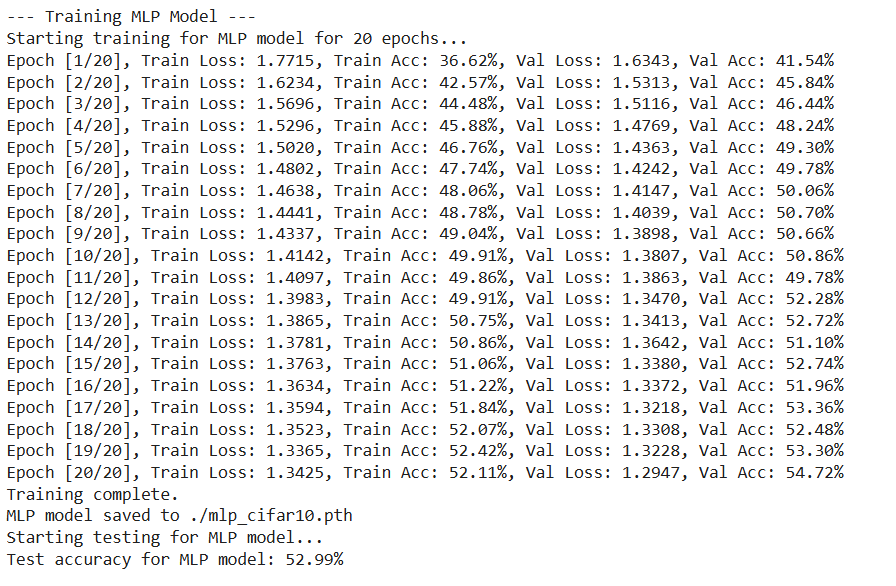
\includegraphics[width=0.9\textwidth]{Screenshots/Ảnh chụp màn hình 2025-05-23 222816.png} % Replace with your image path
    \caption{MLP Training Log}
    \label{fig:mlp_training_log}
\end{figure}

\subsubsection{Learning Curves}
The learning curve graph for MLP shows how the loss and accuracy change throughout training: \\
\textbf{Loss Chart:}
\begin{figure}[H]
    \centering
    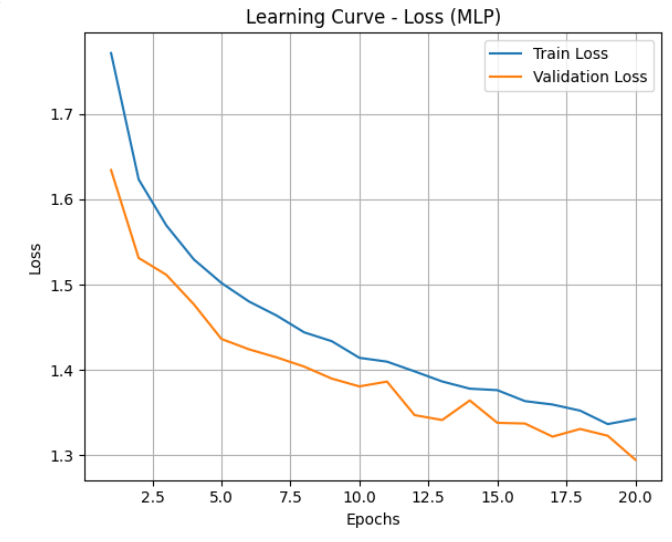
\includegraphics[width=0.7\textwidth]{Screenshots/Ảnh chụp màn hình 2025-05-23 222935.png} % Replace with your image path
    \caption{Learning Curve - Loss (MLP)}
    \label{fig:mlp_loss_chart}
\end{figure}
\textbf{Comment:} The Training Loss decreases over epochs, indicating that the model is learning from the data. However, the Validation Loss tends to decrease slowly and may start to increase slightly in the last epochs, or remain at a large distance from the Training Loss, suggesting overfitting.

\textbf{Accuracy Chart:}
\begin{figure}[H]
    \centering
    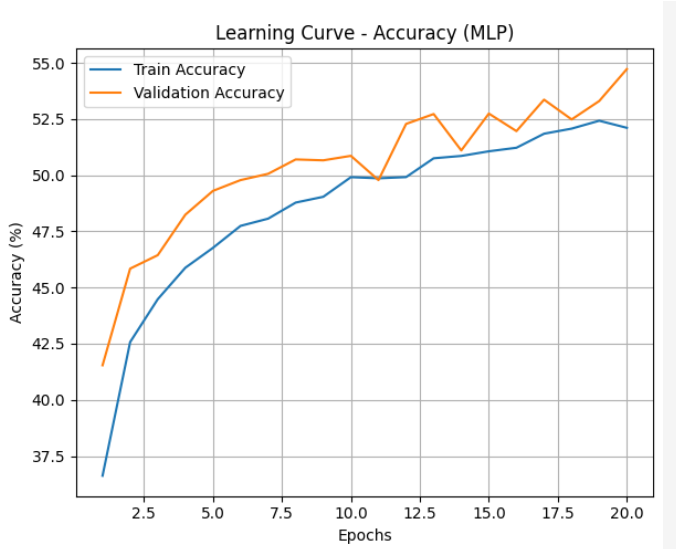
\includegraphics[width=0.7\textwidth]{Screenshots/Ảnh chụp màn hình 2025-05-23 223040.png} % Replace with your image path
    \caption{Learning Curve - Accuracy (MLP)}
    \label{fig:mlp_accuracy_chart}
\end{figure}
\textbf{Comment:} The accuracy on the training set (Train Acc) continues to increase and reaches a fairly high level, while the accuracy on the validation set (Validation Acc) increases more slowly and tends to saturate after the first few epochs. This is also a sign of overfitting, when the model learns too specific examples of the training set.

\subsubsection{Classification Report}
The classification report provides detailed metrics (Precision, Recall, F1-score) for each class and overall on the test set:
\begin{figure}[H]
    \centering
    \hspace*{4cm}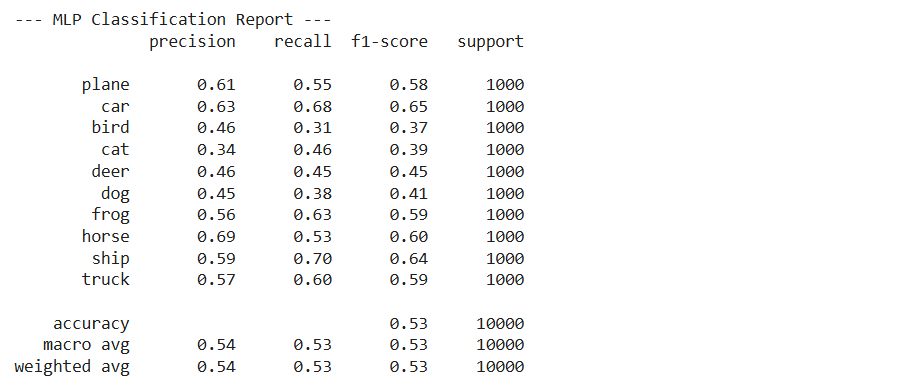
\includegraphics[width=0.8\textwidth]{Screenshots/Ảnh chụp màn hình 2025-05-23 223142.png} % Replace with your image path
    \caption{MLP Classification Report}
    \label{fig:mlp_classification_report}
\end{figure}

\subsubsection{Confusion Matrix}
The confusion matrix visualizes the number of correct and incorrect predictions for each class:
\begin{figure}[H]
    \centering
    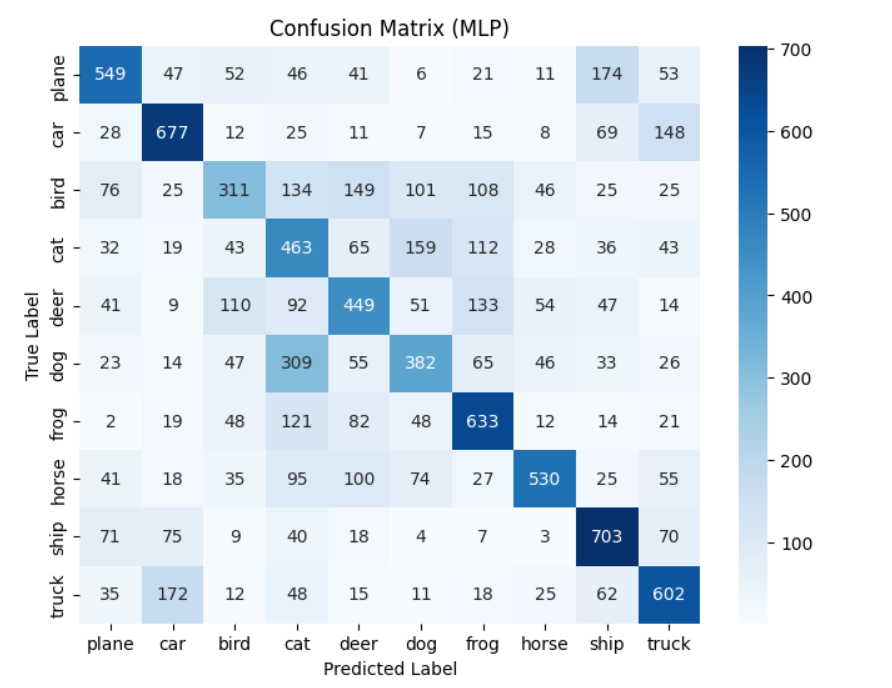
\includegraphics[width=0.8\textwidth]{Screenshots/Ảnh chụp màn hình 2025-05-23 223226.png} % Replace with your image path
    \caption{Confusion Matrix (MLP)}
    \label{fig:mlp_confusion_matrix}
\end{figure}
\textbf{Comment:} The confusion matrix shows that the MLP has difficulty distinguishing classes with similar visual features. Specifically, the number of false predictions between pairs like “cat” and “dog”, or “bird” and “plane” is quite high. The values on the main diagonal (correct predictions) are relatively low for some classes, confirming the limited performance of this model on complex datasets like CIFAR-10.

\subsubsection{Show random predictions and initial comments on MLP performance}
To get a visual idea of the model's predictive ability, we've shown some random images from the test set along with the actual labels and the MLP's predicted labels:

\begin{figure}[H]
    \centering
    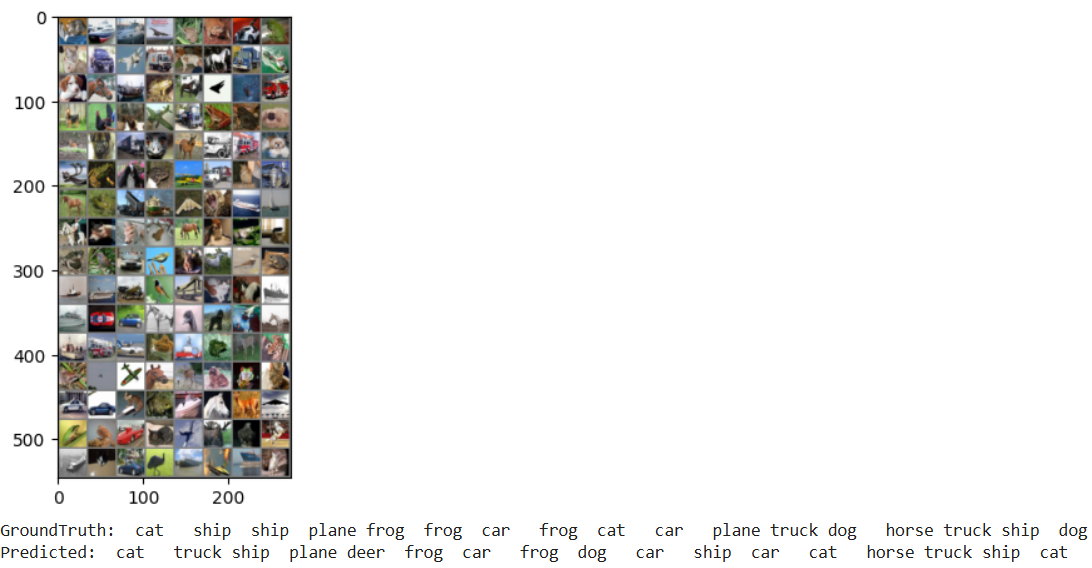
\includegraphics[width=0.9\textwidth]{Screenshots/Ảnh chụp màn hình 2025-05-23 223320.png} % Replace with your image path
    \caption{Random Test Image and MLP Prediction}
    \label{fig:mlp_random_predictions}
\end{figure}
\textbf{Comment:} Observing the images shows that the MLP can correctly predict some obvious objects like “car” or “ship”. However, it frequently makes mistakes with more complex or similar shaped objects like “cat”, “dog”, “bird” or “deer”. This reflects the low overall accuracy and limited feature learning ability of the MLP when processing raw images.

\subsubsection{Save the trained model (Save Model)}
After training, the state (\texttt{state\_dict}) of the MLP model is saved to the \texttt{mlp\_cifar10.pth} file. This allows us to reload the model without retraining, which is useful for future deployment or continued training. Save path: \texttt{./mlp\_cifar10.pth}.

\subsection{CNN model results}
\subsubsection{Training and testing process}
The CNN model was trained for 20 epochs with the same configuration as MLP. Below is the summary training log of each epoch and print test accuracy:
\begin{figure}[H]
    \centering
    \hspace*{2cm}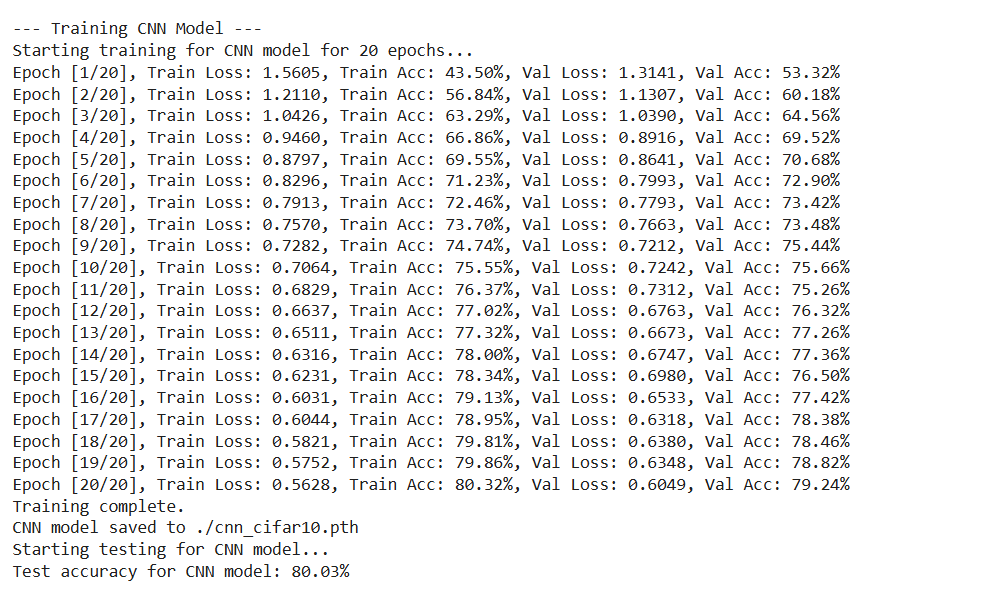
\includegraphics[width=0.9\textwidth]{Screenshots/Ảnh chụp màn hình 2025-05-23 223434.png} % Replace with your image path
    \caption{CNN Training Log}
    \label{fig:cnn_training_log}
\end{figure}

\subsubsection{Learning Curves}
The learning curve graph for the CNN shows a significant improvement in performance:
\textbf{Loss Chart:}
\begin{figure}[H]
    \centering
    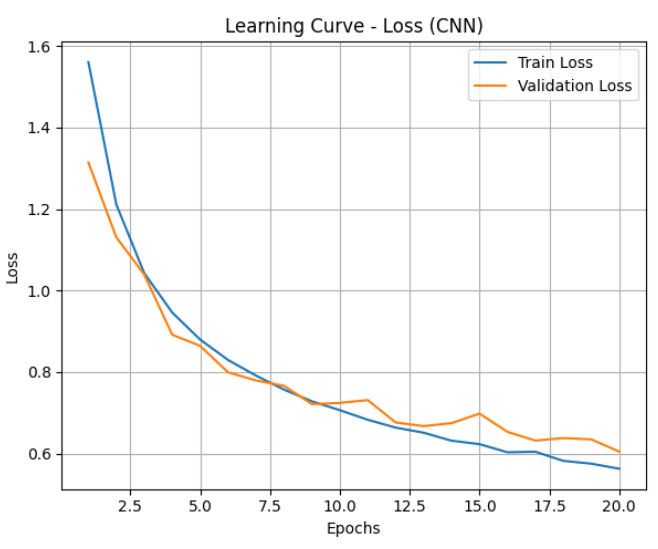
\includegraphics[width=0.7\textwidth]{Screenshots/Ảnh chụp màn hình 2025-05-23 223515.png} % Replace with your image path
    \caption{Learning Curve - Loss (CNN)}
    \label{fig:cnn_loss_chart}
\end{figure}
\textbf{Comment:} The CNN's Training Loss and Validation Loss decrease very quickly and converge to a much lower value than the MLP. The gap between the two lines is also significantly smaller, indicating that the model learns efficiently and has good generalization ability without much overfitting.

\textbf{Accuracy Chart:}
\begin{figure}[H]
    \centering
    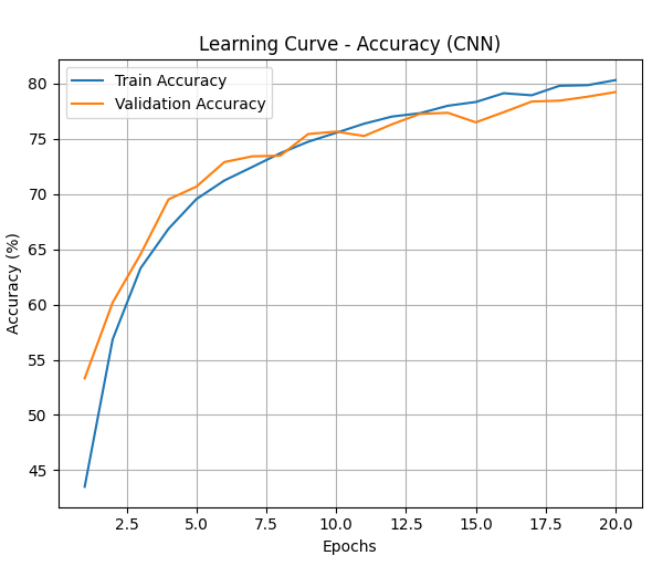
\includegraphics[width=0.7\textwidth]{Screenshots/Ảnh chụp màn hình 2025-05-23 223550.png} % Replace with your image path
    \caption{Learning Curve - Accuracy (CNN)}
    \label{fig:cnn_accuracy_chart}
\end{figure}
\textbf{Comment:} The accuracy on both the training and validation sets of the CNN increases rapidly and reaches very high levels. The validation accuracy curve is almost parallel and close to the training curve, indicating that the model is learning well and generalizing effectively on new data.

\subsubsection{Classification Report}
The report details the CNN performance on the test set:
\begin{figure}[H]
    \centering
    \hspace*{3.5cm}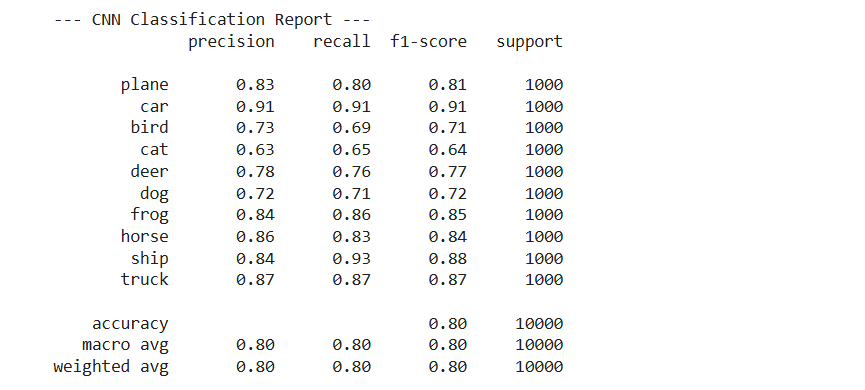
\includegraphics[width=0.8\textwidth]{Screenshots/Ảnh chụp màn hình 2025-05-23 223634.png} % Replace with your image path
    \caption{CNN Classification Report}
    \label{fig:cnn_classification_report}
\end{figure}

\subsubsection{Confusion Matrix}
CNN confusion matrix:
\begin{figure}[H]
    \centering
    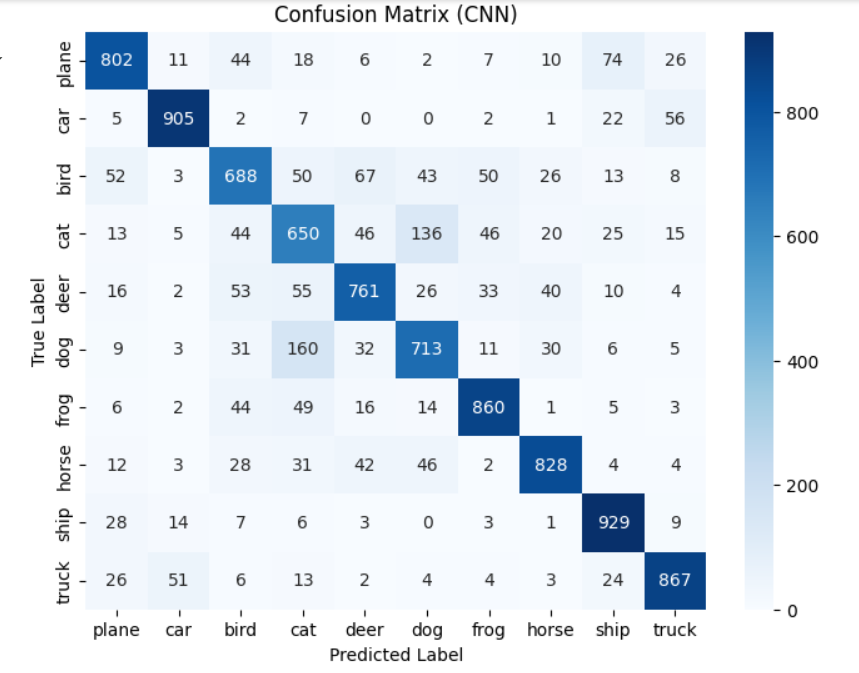
\includegraphics[width=0.8\textwidth]{Screenshots/Ảnh chụp màn hình 2025-05-23 223731.png} % Replace with your image path
    \caption{Confusion Matrix (CNN)}
    \label{fig:cnn_confusion_matrix}
\end{figure}
\textbf{Comment:} The CNN confusion matrix shows that the values on the main diagonal (correct predictions) are very high for most of the classes. This confirms the CNN's ability to classify accurately. Although there are still some small confusions between similar classes like "cat" and "dog", or "bird" and "plane", the number of these confusions is significantly less than that of MLP.

\subsubsection{Random Prediction Display and Initial Comments on CNN Performance}
Show some random images from the test set along with the actual label and the CNN's predicted label:

\begin{figure}[H]
    \centering
    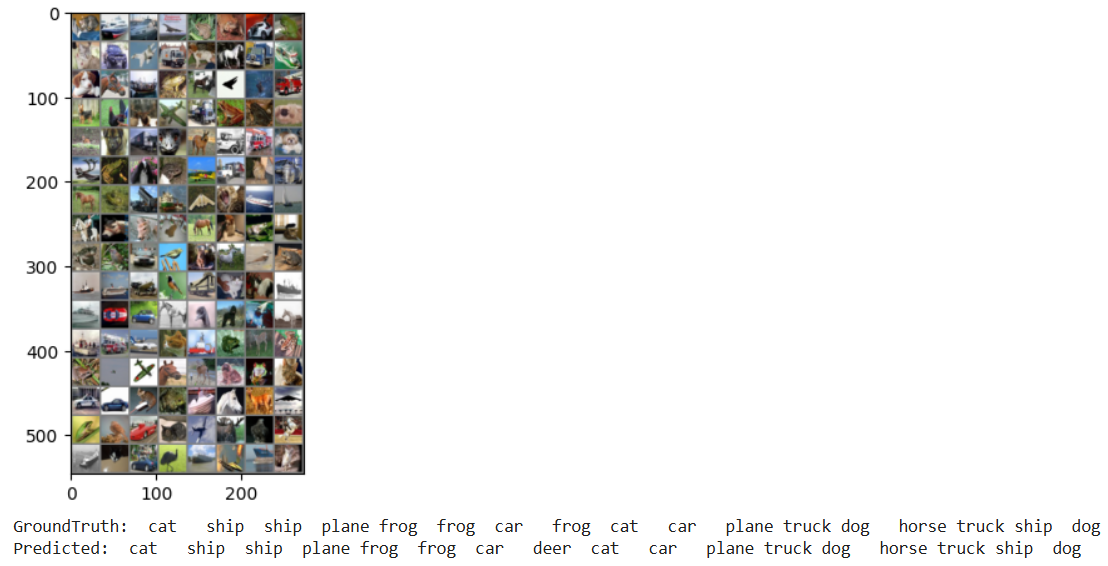
\includegraphics[width=0.9\textwidth]{Screenshots/Ảnh chụp màn hình 2025-05-23 223812.png} % Replace with your image path
    \caption{Random Test Image and CNN Prediction}
    \label{fig:cnn_random_predictions}
\end{figure}
\textbf{Comment:} CNN predictions on random images are much more accurate than MLP. Most of the objects, whether animals or vehicles, are classified correctly. This illustrates the powerful feature extraction and efficient classification capabilities of the CNN architecture.

\subsubsection{Save the trained model (Save Model)}
After training, the state (\texttt{state\_dict}) of the CNN model has also been saved to the \texttt{cnn\_cifar10.pth} file. This storage is important to reuse the model without having to train it from scratch. Save path: \texttt{./cnn\_cifar10.pth}.

\subsection{Comparison and discussion of results between MLP and CNN}
\subsubsection{Overview comparison table}
To summarize, here is a table comparing the final accuracy of the two models on the test set:

\begin{longtable}{|p{0.3\textwidth}|p{0.4\textwidth}|}
\caption{Comparison of Test Accuracy for MLP and CNN}
\label{tab:comparison_accuracy} \\
\toprule
\textbf{Model} & \textbf{Test Set Accuracy} \\
\midrule
MLP & 52.99\% \\
CNN & 80.03\% \\
\bottomrule
\end{longtable}

\subsubsection{Analysis of causes of performance differences}
The significant performance difference between MLP and CNN in the CIFAR-10 image classification problem can be explained by the following core reasons:
\begin{itemize}
    \item \textbf{Image data nature:} Images have significant spatial structure (e.g. neighboring pixels have close relationships).
    \begin{itemize}
        \item \textbf{MLP:} Processes an image by flattening it into a 1D vector. This process completely loses information about the relative positions between pixels. Therefore, MLPs have to learn from scratch the complex relationships between spatially unrelated pixels, making it difficult to extract meaningful features from the image.
        \item \textbf{CNN:} The convolutional layers of a CNN are designed to take advantage of this spatial structure. They use filters (kernels) to scan through the image, detecting local patterns (like edges, textures, shapes). Sharing the weights of these filters across the entire image makes the CNN much more efficient at learning image features and also greatly reduces the number of parameters to learn.
    \end{itemize}
    \item \textbf{Automatic feature extraction capabilities:}
    \begin{itemize}
        \item \textbf{MLP:} As a “shallow learning” network, the hidden layers of an MLP are not capable of automatically learning high-level features from raw data. It mainly learns simple linear or nonlinear relationships between input pixels.
        \item \textbf{CNN:} CNNs are capable of building a hierarchy of features. Early convolutional layers learn low-level features (e.g., edges, lines), while deeper layers combine these features to create higher-level features (e.g., eyes, ears, wheels). This ability to extract features automatically and hierarchically is key to CNNs' superior performance in computer vision tasks.
    \end{itemize}
    \item \textbf{Translation Invariance:} The Max Pooling layers in CNN make the model less sensitive to small displacements of objects in the image. That is, no matter where the object appears in the image, the CNN is still able to recognize it. MLPs do not have this property; if an object moves position in the image, the input pixels will change significantly, and the MLP needs to relearn the pattern at the new position.
    
\end{itemize}

\newpage
\section{CONCLUSION}
This paper has successfully performed image classification on the CIFAR-10 dataset by constructing and comparing two neural network models: Multi-Layer Perceptron (MLP) and Convolutional Neural Network (CNN). The main results can be summarized as follows:
\begin{itemize}
    \item \textbf{MLP Model:} The accuracy achieved on the test set is 52.99\%. Although the model learns and the loss decreases, and the accuracy increases over epochs, the overall performance is limited. The learning curves show early saturation, and the classification report indicates difficulty in distinguishing classes with similar visual features (e.g., cat, dog, bird).
    \item \textbf{CNN model:} The accuracy achieved on the test set is 80.03\%. This is a significant improvement, outperforming MLP by 27.04\%. The CNN learning curves demonstrate fast learning, stability, and good generalization ability. The classification report and confusion matrix show that the CNN has a better ability to discriminate between classes, significantly reducing confusion errors.
\end{itemize}
This clear difference in performance confirms the superiority of CNNs in computer vision problems. CNNs effectively exploit the spatial structure of images through convolutional layers, weight sharing mechanisms, and the ability to learn hierarchical features, which MLPs cannot do due to data flattening.

\end{document}